\documentclass{article}

\title{Supply and Demand Journal}
\author{Wellen}
\date{\today}

\usepackage[utf8]{inputenc}
\usepackage[margin=1in]{geometry}
\usepackage{url, appendix, pdfpages, subcaption} %for inputting urls, appendices, outside docs, and placing multiple pictures in the same figure
%http://blog.bharatbhole.com/inserting-pages-from-an-external-pdf-document-within-a-latex-document/
\usepackage{float} %[H] tells LaTeX you absolutely want an image there
\usepackage{fancyhdr, enumitem}
\newcommand{\compresslist}{ % Define a command to reduce spacing within itemize/enumerate environments, this is used right after \begin{itemize} or \begin{enumerate}
	\setlength{\itemsep}{0pt}
	\setlength{\parskip}{0pt}
	\setlength{\parsep}{10pt}
}
\usepackage{amsmath, amssymb, mathrsfs, dsfont, amsthm,  cancel}
\usepackage[mathscr]{eucal} %for getting less bold and swirlier math scripts
\usepackage{graphicx, tikz, wrapfig} %for figures, figure creation, and haveing text to the left of a figure
\allowdisplaybreaks[1]

\usepackage{titlesec}
%\titlespacing*{\subsubsection}{0pt}{0\baselineskip}{\baselineskip}

%Places the title information in the header
\makeatletter         
%\def\@maketitle{{\bfseries\@title}\\ \@author \\ \@date }


%%%%%%%%%%%%%%%%%%%%%%%%%%%%%%%%%%%%%%%%%%%%%%%%%%%%%%%%%%%%%%%%%%%%%%
%
%								MACROS
%
%%%%%%%%%%%%%%%%%%%%%%%%%%%%%%%%%%%%%%%%%%%%%%%%%%%%%%%%%%%%%%%%%%%%%%

%                   Brackets and Parenthesis

\newcommand{\<}{\langle}
\renewcommand{\>}{\rangle}
\renewcommand{\(}{\left(}
\renewcommand{\)}{\right)}
\renewcommand{\[}{\left[}
\renewcommand{\]}{\right]}

%                   Math Blackboard Bold Symbols

\newcommand\Cb{\mathds{C}}
\newcommand\Eb{\mathds{E}}
\newcommand\Fb{\mathds{F}}
\newcommand\Gb{\mathds{G}}
\newcommand\Pb{\mathds{P}}
\newcommand\Qb{\mathds{Q}}
\newcommand\Rb{\mathds{R}}
\newcommand\Zb{\mathds{Z}}
\newcommand\Nb{\mathds{N}}
\newcommand\Vb{\mathds{V}}

%                   mathscr symbols

\newcommand\Ac{\mathscr{A}}
\newcommand\Bc{\mathscr{B}}
\newcommand\Cc{\mathscr{C}}
\newcommand\Dc{\mathscr{D}}
\newcommand\Ec{\mathscr{E}}
\newcommand\Fc{\mathscr{F}}
\newcommand\Gc{\mathscr{G}}
\newcommand\Hc{\mathscr{H}}
\newcommand\Lc{\mathscr{L}}
\newcommand\Mc{\mathscr{M}}
\newcommand\Nc{\mathscr{N}}
\newcommand\Oc{\mathscr{O}}
\newcommand\Pc{\mathscr{P}}
\newcommand\Qc{\mathscr{Q}}
\newcommand\Sc{\mathscr{S}}
\newcommand\Kc{\mathscr{K}}
\newcommand\Jc{\mathscr{J}}
\newcommand\Xc{\mathscr{X}}
\newcommand\Yc{\mathscr{Y}}
\newcommand\Zc{\mathscr{Z}}

%                   shortcuts for greek letters

\newcommand\eps{\epsilon}
\newcommand\om{\omega}
\newcommand\Om{\Omega}
\newcommand\sig{\sigma}
\newcommand\Sig{\Sigma}
\newcommand\Lam{\Lambda}
\newcommand\gam{\gamma}
\newcommand\Gam{\Gamma}
\newcommand\lam{\lambda}
\newcommand\del{\delta}
\newcommand\Del{\Delta}
\newcommand\Chi{\mathcal{X}}

%                   Letters with bars

\newcommand\Wb{\overline{W}}
\newcommand\Mb{\overline{M}}
\newcommand\Xb{\overline{X}}
\newcommand\Yb{\overline{Y}}
\newcommand\Sb{\overline{S}}
\newcommand\Pbb{\overline{\Pb}}
\newcommand\Ebb{\overline{\Eb}}
\newcommand\Acb{\bar{\Ac}}
\newcommand\ab{\overline{a}}
\newcommand\bb{\overline{b}}
\newcommand\hb{\overline{h}}
\newcommand\xb{\bar{x}}
\newcommand\yb{\bar{y}}
\newcommand\zb{\bar{z}}
\newcommand\Ab{\bar{\Ac}}
\newcommand\vb{\bar{v}}
\newcommand\ub{\bar{u}}
\newcommand\qb{\bar{q}}
\newcommand\pb{\bar{p}}
%\newcommand\Vb{\bar{V}}
\newcommand\rhob{\bar{\rho}}
\newcommand\IIb{\bar{\II}}
\newcommand\LLb{\bar{\LL}}
\newcommand{\psib}{\bar{\psi}}
\newcommand{\etab}{\bar{\eta}}
\newcommand{\xib}{\bar{\xi}}

%                   Letters with underlines

\newcommand\Wu{\underline{W}}
\newcommand\Xu{\underline{X}}
\newcommand\Mu{\underline{M}}

%                   Vectors (bolded)

\newcommand\Av{\mathbf{A}}
\newcommand\Fv{\mathbf{F}}
\newcommand\xv{\mathbf{x}}
\newcommand\bv{\mathbf{b}}
\newcommand\pv{\mathbf{p}}
\newcommand\qv{\mathbf{q}}
\newcommand\ev{\mathbf{e}}
\newcommand\yv{\mathbf{y}}
\newcommand\zv{\mathbf{z}}
\newcommand\Yv{\mathbf{Y}}
\newcommand\Hv{\mathbf{H}}
\newcommand\Cv{\mathbf{C}}
\newcommand\mv{\mathbf{m}}
\newcommand\etav{\boldsymbol\eta}
\newcommand\piv{\boldsymbol \pi}
\newcommand\muv{\boldsymbol \mu}
\newcommand\Sv{\textbf S}
\newcommand\Qv{\textbf Q}
\newcommand\zev{\textbf 0}

%                   Letters with Hats

\newcommand\Pbh{\widehat{\Pb}}
\newcommand\Ebh{\widehat{\Eb}}
\newcommand\Qh{\widehat{Q}}
\newcommand\Ih{\widehat{I}}
\newcommand\pih{\widehat{\pi}}
\newcommand\Pih{\widehat{\Pi}}
\newcommand\varphih{\widehat{\varphi}}
\newcommand\Wh{\widehat{W}}
\newcommand\Fh{\widehat{F}}
\newcommand\Yh{\widehat{Y}}
\newcommand\Ah{\widehat{\Ac}}
\newcommand\uh{\widehat{u}}
\newcommand\Uh{\widehat{U}}
\newcommand\vh{\widehat{v}}
\newcommand\fh{\widehat{f}}
\newcommand\Hh{\widehat{H}}
\newcommand\hh{\widehat{h}}
\newcommand\Bh{\widehat{B}}
\newcommand\etah{\widehat{\eta}}
\newcommand\Lh{\widehat{L}}

%                   Letters with Tildes

\newcommand\Ebt{\widetilde{\Eb}}
\newcommand\Pbt{\widetilde{\Pb}}
\newcommand\Act{\widetilde{\Ac}}
\newcommand\Lct{\widetilde{\Lc}}
\newcommand\Gct{\widetilde{\Gc}}
\newcommand\Xct{\widetilde{\Xc}}
\newcommand\Yct{\widetilde{\Yc}}
\newcommand\Zct{\widetilde{\Zc}}
\newcommand\Mt{\widetilde{M}}
\newcommand\Wt{\widetilde{W}}
\newcommand\Bt{\widetilde{B}}
\newcommand\Nt{\widetilde{N}}
\newcommand\Xt{\widetilde{X}}
\newcommand\xt{\widetilde{x}}
\newcommand\ut{\widetilde{u}}
\newcommand\kappat{\widetilde{\kappa}}
\newcommand\at{\widetilde{a}}
\newcommand\Gamt{\widetilde{\Gam}}
\newcommand\Pct{\widetilde{\Pc}}


%         Theorem environments

\newtheoremstyle{mine}% name of the style to be used
  { }% measure of space to leave above the theorem. E.g.: 3pt
  { }% measure of space to leave below the theorem. E.g.: 3pt
  { }% name of font to use in the body of the theorem
  { }% measure of space to indent
  { }% name of head font
  { }% punctuation between head and body
  { }% space after theorem head; " " = normal interword space
  {\thmname{\textbf{#1}}\thmnumber{\textbf{ #2}}:\thmnote{ #3}\\}% Manually specify head

\theoremstyle{mine}
\newtheorem{thm}{Theorem}[section]
\newtheorem{cor}[thm]{Corollary}
\newtheorem{prop}[thm]{Proposition}
\newtheorem{defn}[thm]{Definition}
\newtheorem{rmk}[thm]{Remark}
\newtheorem{lem}[thm]{Lemma}
\newtheorem{assumption}[thm]{Assumption}


%                   other macros

\newcommand{\dd}{\partial}
\newcommand{\ind}{\perp \! \! \! \perp}
\newcommand\ii{\mathtt{i}}
\renewcommand\d{\mathrm{d}}
\newcommand\ee{\mathrm{e}}
\newcommand\BS{\textrm{BS}}
\newcommand\ko{\mathrm{ko}}
\newcommand\ki{\mathrm{ki}}
\newcommand\rb{\mathrm{rb}}
\newcommand\eu{\mathrm{eu}}

%          other


\newcommand\Ib{\mathds{1}}
\renewcommand\Re{\operatorname{Re}}
\renewcommand\Im{\operatorname{Im}}
\newcommand{\nuba}[1]{\overline{\nu_{#1}^\ast}}
\newcommand{\tab}{\hspace{.4 in}}
\newcommand{\enter}{\vspace{.15 in}}
\newcommand{\fa}{\forall}
\newcommand{\tf}{\therefore}
\newcommand{\indep}{\raisebox{0.05em}{\rotatebox[origin=c]{90}{$\models$}}}
\newcommand{\nth}[2]{#1^{\text{\tiny #2}}}
\newcommand{\xRightarrow}[2][]{\ext@arrow 0359\Rightarrowfill@{#1}{#2}}
\newcommand{\myeq}[1]{\mathrel{\overset{\makebox[0pt]{\mbox{\small {#1}}}}{=}}}
\newcommand{\since}{\reflectbox{\rotatebox[origin=c]{180}{$\therefore$}}}
\makeatother


\begin{document}

\begin{figure}%
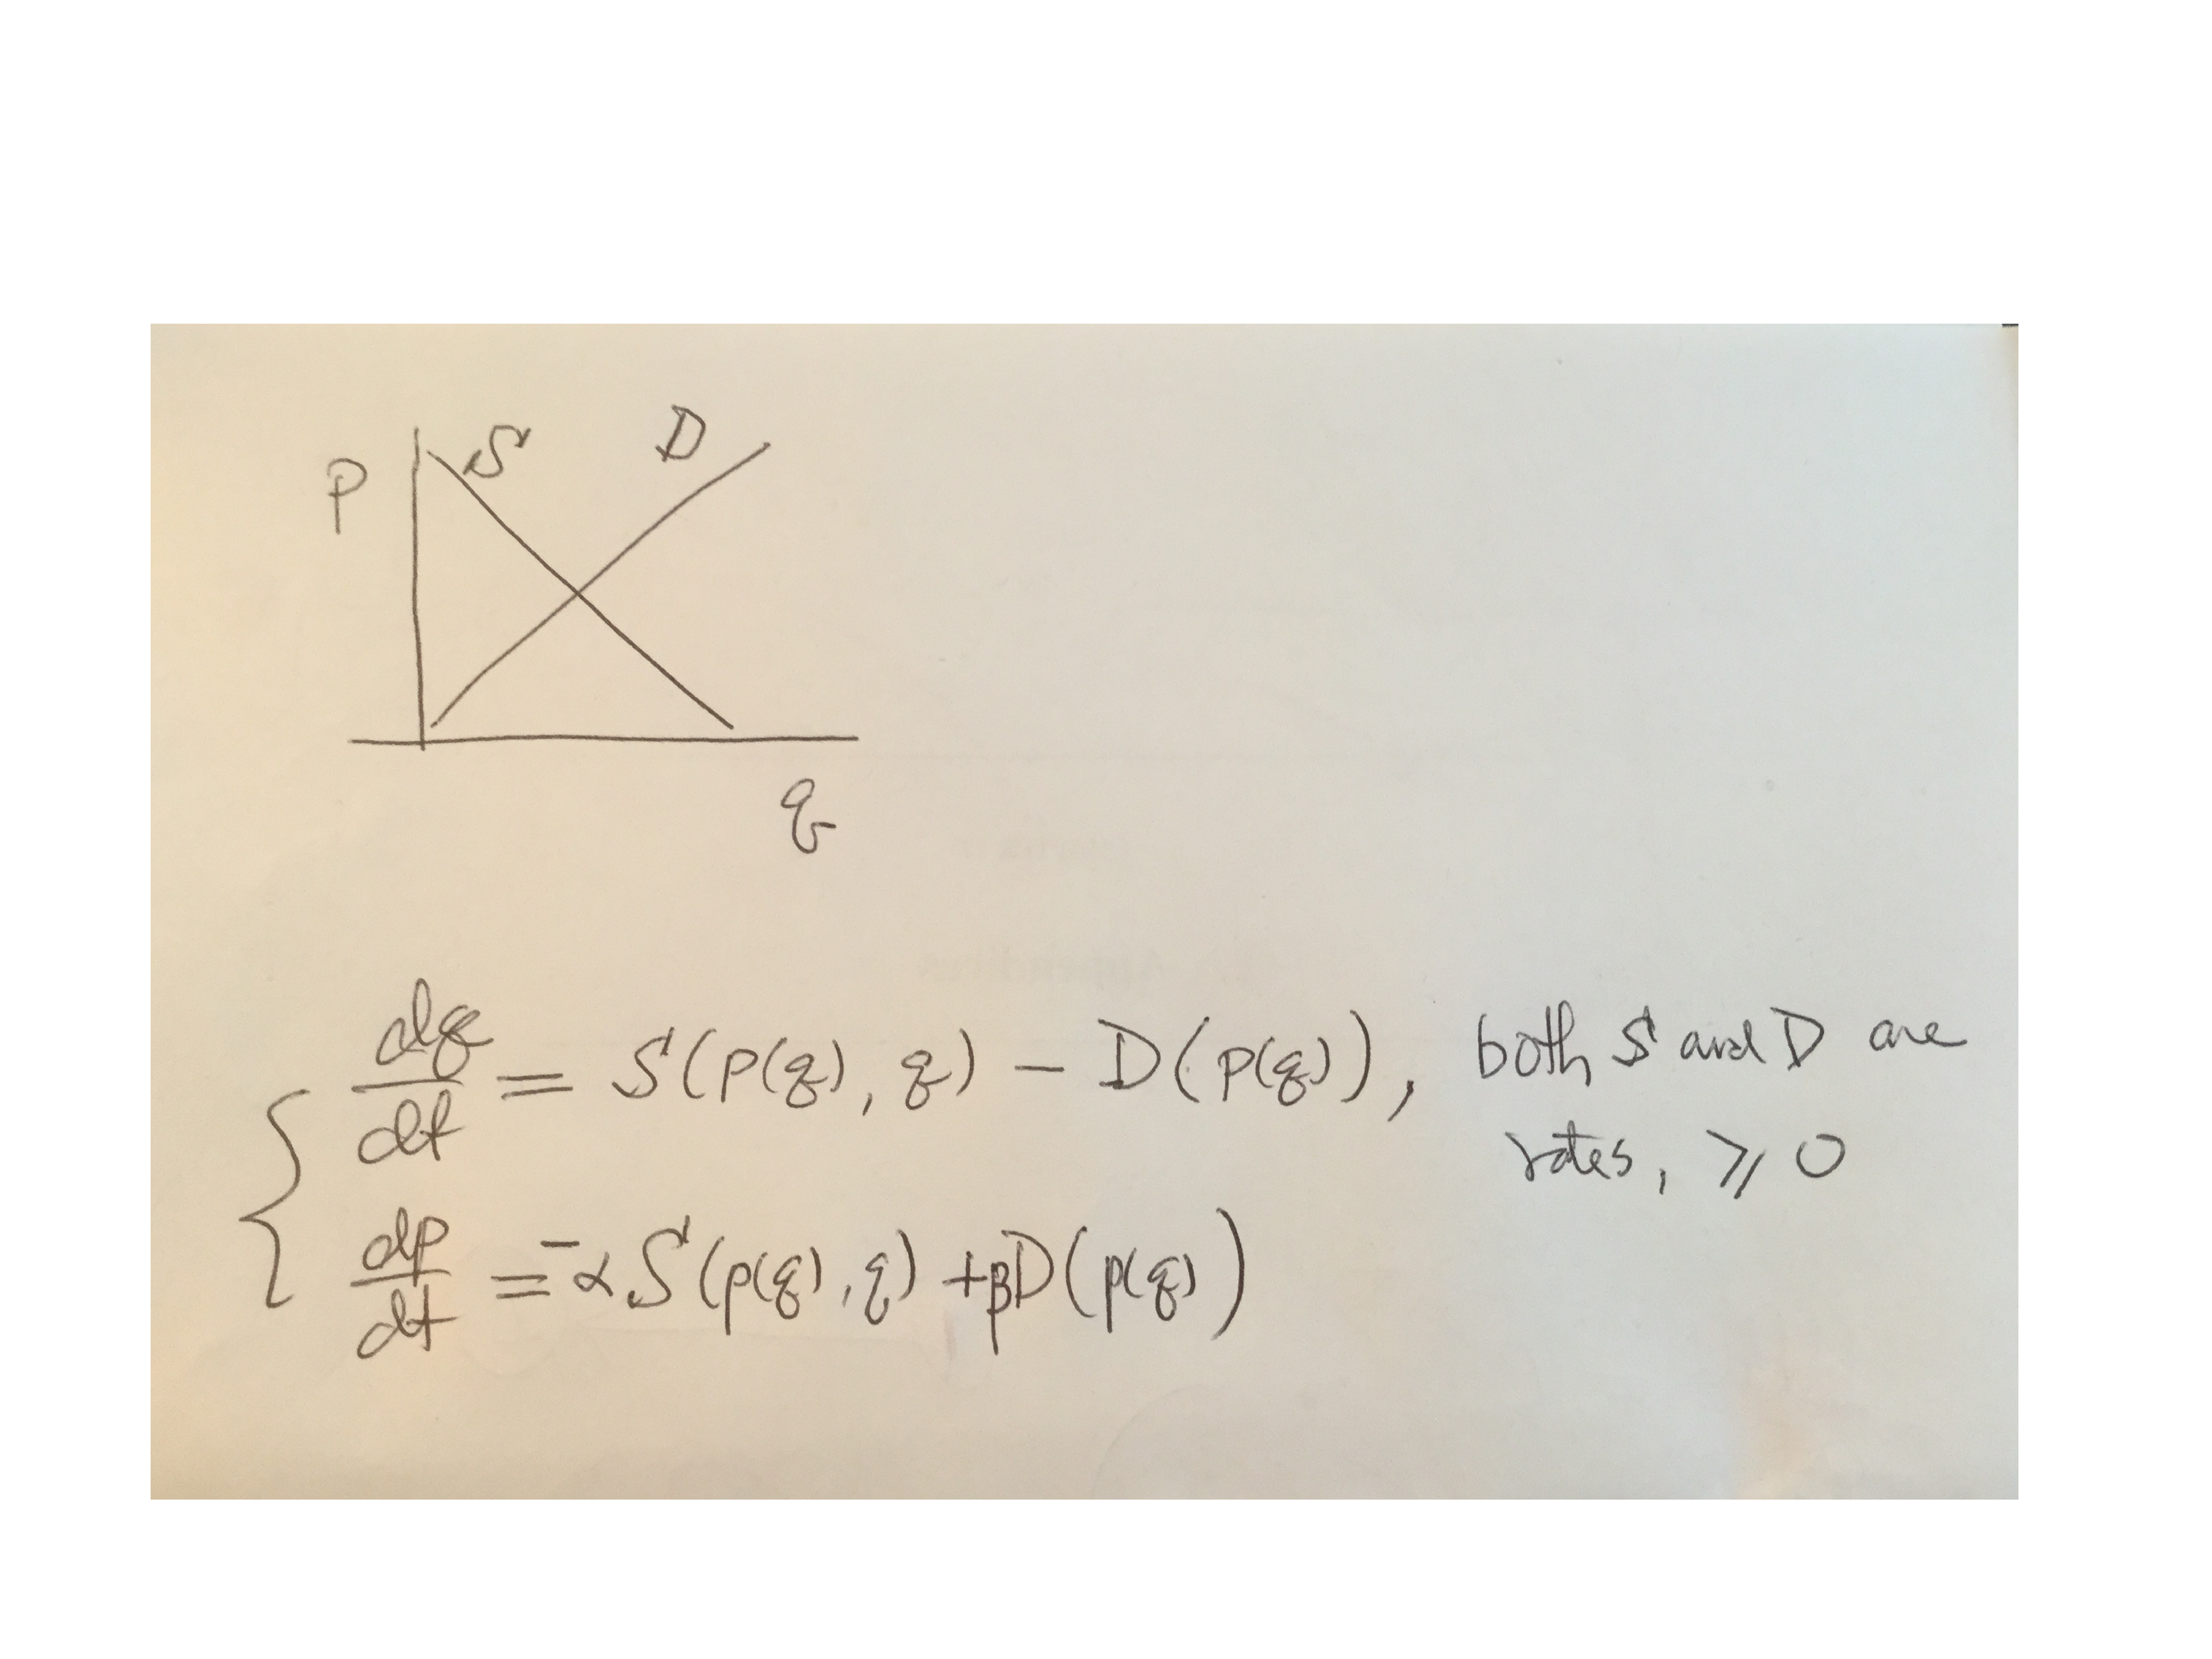
\includegraphics[width=\columnwidth]{Figures/IMG_0977_HongsSnD.pdf}%
\caption{The System of ODE's that Hong created to describe supply and demand}%
\label{hong}%
\end{figure}

``Does it make sense?  If not why?  If yes, has anyone already done that? ''

I also want to know if economics is weak chaos (bounded).

In which $\alpha$ and $\beta$ are two positive constants that convert the rate of change in q to that or rate of change in p.

\section{Has anyone already done that?}
So I answered this question first. I had a meeting with Matt and Hong 02/27/20 where they made clear in person that I was supposed to be doing this at the same time as answering the other two questions. Now, rereading what Hong sent me before Winter Break, I think it also implied that if not at the same time then after. 

The first order simple ODE has been studied extensively by economists, and I looked at and presented one form of this already. Clower wrote a paper analyzing the meaning of the first order dynamical system in regards to the basic supply and demand curves, and disequilibrium theory has done some work with this. 

What has not been done, is the analysis of a second order description of the system that describes the state of depression in the economy as an equilibrium as well. This is the model that I want to work on.

First thing suggested to check is whether this reproduce the figure in
\url{https://en.wikipedia.org/wiki/Supply_and_demand},'' which is more or less Fig \ref{hong}. What I found in the literature is that this picture is exactly how the current dynamical systems models were made. Rather than checking in retrospect, they defined the calculus analysis already inherent there as the dynamics. My goal is to start from scratch as best I can and then see how that compares to previous models


\section{First Model from Lit}

	A Simple Dynamical System - \underline{Economic Dynamics: Phase Diagrams and Their Economic Application} by Ronald Shone
	\begin{itemize}
		\item In a typical economy the price is set by producers, and then adjusted based on observations
		\item This means typically what is observed in the economy is \emph{dynamic adjustment process}
		\item To not just discuss that price will increase or decrease so that supply matches demand, we can examine the underlying dynamics behind price movement
	\end{itemize}
	
	\textbf{Model 1}
	\begin{align*}
		q_d =& a - bp && b >& 0\\ %linear equation of demand
		q_s =& c + fp && f >& 0 \\ %linear equation of supply
		\frac{\d p}{\d t} =& \alpha(q_d - q_s) = \alpha(b+f)p - \alpha(a-c) && \alpha >& 0
	\end{align*}
	%solution is p(t) = \frac{a-c}{b+f} + \[p_0 - \(\frac{a-c}{b+f}\)\]e^{-\alpha(b+f)t}
	%p(0) = p_0
	$q_d,\ q_s,\ \&\ p$ are continuous functions of time.

Supply and Demand
	\begin{figure}
		\centering
			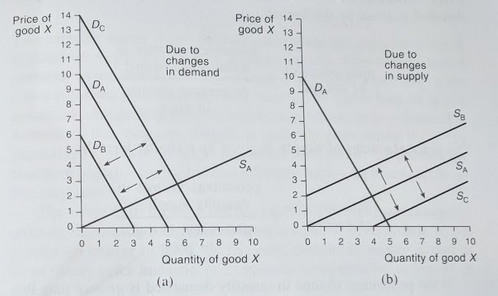
\includegraphics{Figures/SnD.png}
		\caption{Walrasian supply and demand}
	\end{figure}
	
	At equilibrium we have that $\frac{\d p}{\d t} = \alpha(q_d - q_s) = 0 \ \Rightarrow \ p^* = \frac{a-c}{b+f}$ and $q^* = \frac{af + bc}{b+f}$

Without Stocks
	\begin{assumption}
		In disequilibrium the short side of the market is transacted. In other words only current supply is available to fill demand and there is no stock of goods.
	\end{assumption}
	\begin{itemize}
		\item Excess demand gives a signal for producers to increase supply and price
		\item Excess supply gives signal for producers to decrease supply and price
		\begin{itemize}
			\item It says nothing about what happens to excess goods...
		\end{itemize}
	\end{itemize}	

With Stocks
	\begin{assumption}
		Stocks are sufficient to meet demand at any price, and price adjusts to changes in stock levels.
	\end{assumption}
	\textbf{Model 2}
	\begin{align*}
		i =& i_0 + \int_0^t{q_s - q_d}\d t\\
		\frac{\d i}{\d t} = & q_s - q_d \\
		\frac{\d p}{\d t} =& -\alpha\frac{\d i}{\d t} = \alpha(q_d - q_s) && \alpha > 0
	\end{align*}	
	\begin{itemize}
		\item The price path solution is the same
		\item However now we allow for the quantity traded to increase s.t. $q(t) = q_d(t)\ \fa\ p$
	\end{itemize}

Further systems
	\begin{itemize}
		\item This approach can be applied to labor markets with and without flexible wages
		\item These labor models are then related to supply and demand in that decreases in price indicate decreases in labor demand
		\begin{itemize}
			\item In sticky wage models we make assumptions about how demand once again determines dynamics
			\item There are also assumptions accounting for how there are asymmetric adjustments: wages increase faster than they decrease
		\end{itemize}
		\item Discretizing the time flow leads to what is called the cobweb model
	\end{itemize}


%%%%%%%%%%%%%%%%%%%%%%%%%%%%%%%%%%%%%%%%%%%%%%%%%%%%%%%%%%%%%%%%%%%%%%%%%%%%%%%%%%%%%%%%%%%%%%%%%%%%%%%%%%%%%%%%%%%%%%%%%%%%%%%%%%%%%%%%
\section{My Model}
Could also be a markov chain that describes the system.

\subsection{Things that go into supply and demand}
\begin{itemize}
	\item supply
	\item demand
	\item price
	\item quantity
	\item current stock
	\item expiration of stock (rate of decay of item, often idealized to infinity or zero)
	\item utility - useful, time it takes to acquire, ease of use, etc.
	\item available substitutions
	\item budget, including savings ( so expected much less than income because housing and so on)
	\item coolness factor
	\item elasticity (assumed linear or is it non-linear?)
\end{itemize}

\subsection{How do supply and demand interact?}
Something interesting that I always thought was left out is rarity. It is really obvious in trading cards, but also in Grey Poupon mustard. Something can be more expensive and that attracts people to it perhaps because of ideas of luxury. Because of this sort of thing, I do not believe that the interaction between supply and demand is linear, so then the question is what kind of non-linearity makes sense. 

I do not believe it would be oscillatory, so the question is what order polynomial and how does it relate? 
Thinking about AMATH 568 for non-linear ODE's, we work almost entirely with non-linear second order ODE's. Here we have been working with second order ODE's, so I need to think more about how this translates into real world systems. Also sometimes one of our terms has a very small constant out in front. For example what we have below is a second order ODE with a very small damping term. 
\begin{align*}
	-y''[q] - \eps y'[q] +y[q] = 0
\end{align*}
Since $y''[q]$ has an opposing sign to $y[q]$ we may think of the exponential function as our ansatz. The inclusion of the damping term would keep our solution from shooting off to $\infty$. 

Supply and Demand would also be positively correlated. As demand increases supply will increase to match, but less than the quantity demanded, since the price should also be able to increase. This is in an idealized market of course, since if there are competitors, that could keep a company from raising there prices. However, a company will never supply more than the amount demanded since that will drive down prices and thus profit margin, while also increasing stocks leading to reduced profit in the future. When demand quantity decreases we would then expect the supply quantity to decrease more than this, for similar reasons to why it would increase less than with demand increase. We can call this amount of disconnect in change $\delta$ so that we have $\frac{\d q_S}{\d t} \approx (1-\delta)q_d$.

From macroeconomic textbooks we have that 
\begin{align}
	\dot{q}_S = &  c_1 q_D + (\frac{dS}{dq} - \frac{dD}{dq})^{-1}\dot{q}_D \\
	& \ \ \ +\eps\ddot{q}_D %\label{predict_demand}
\end{align}
But from this equation we come to the big question of what $\frac{dS}{dq}$ and $\frac{dD}{dq}$ mean. So perhaps it is still useful to call this term $(1-\delta)$ where we can theoretically understand $\delta$ as the inverse of the spread between what the producers and the consumers theoretically expect for that quantity of goods in the market. An interesting note is that for linear systems the amount that $\dot{q}_S$ changes does not depend on if the change in $q_D$ was positive or negative.

Further, is it possible that in an attempt to predict the necessary supply in the future the company adds on a second derivative term such as \eqref{predict_demand}? 
It would be optimizing in that if they expect things to change quickly, they can try not to run out of stock in stores. This may be especially relevant for the case of perishable goods where rather than always being behind demand until it reaches a equilibrium, trying to be ahead and always have supplied what the consumers will purchase. This would likely need an unknown constant in front of the term that is less than one (it probably has less cost associated to under-perform still). 

We also want to look into how the quantity demanded changes changes over time. I believe as a consumer, that this will be based mostly on the price, where $p$ is the transaction price taking place in the market. There is also something to be said for ease of access and rarity of the goods, so I believe that a positive quadratic term makes sense for the supply available effecting the quantity demanded. I argue that change in quantity supplied is not noticeable to a consumer. Either the store has the good or it does not, I have no idea what others are up to. Thus the change in quantity supplied term is left out. 
\begin{equation}
		\dot{q}_D = - c_1 \dot{p} - c_2(q_S-c_3)^3
\end{equation}

In this system we can assume that companies may change their supply without a large effect on consumption, as long as the consumers can still easily access a good (or highly value the rarity of it which is handled in $c_3$).

Something else that I want to pay attention to is not only the constant shifts in supply and demand curves (think shifting the intercept), but also the non-linear shifts in slope. I have not analyzed a case like that yet.

\subsubsection{Taking Stocks of Goods into Account}
The stock of excess supplied goods also needs to be taken into account. This is only relevant for the case of non-perishable goods, just as I would guess that the second derivative term is only relevant for the case of perishable goods. Do companies want at least a certain amount stockpiled? The only difference in the model is that companies would make less money, so we can ignore this in terms of understanding the dynamics. One major difference is that the as stockpiles grow, prices tend to drop as a way of clearing them out. So it's not just about the amount supplied, but the amount in total available that determines changes in price. We definitely know that 
\begin{equation*}
	\dot{b} = q_s - q_d
\end{equation*}



%-------------------------------------------------------------------------------------------------------------------------------------------------------------------
\section{Demand Functions}
See document JointDistributionOfUtility.pdf


%%%%%%%%%%%%%%%%%%%%%%%%%%%%%%%%%%%%%%%%%%%%%%%%%%%%%%%%%%%%%%%%%%%%%%%%%%%%%%%%%%%%%%%%%%%%%%%%%%%%%%%%%%%%%%%%%%%%%%%%%%%%%%%%%%%%%%%%%%%%%%%%%%%%%%%%%%%%%%%%%%%%
\section{Trust}
Something that I am interested in adding in later on to the model is in regards to viewing the supply and demand system as a cycle of interactions influencing price influencing interactions and so on, as discussed in Debreu's ``Theory of Value.'' In this system I think it is important to include something that translates to \textbf{trust}. Since for the interactions it would make most sense for a probabilistic approach to how much is purchased/at what price (I'm thinking Alan Kirman ``Complex Economics'' Ch.3 on fish markets). Trust would be encompassed in that probability of interaction, the more that the consumer has interacted with the vendor, or maybe even interacted with others that trust the vendor, the higher the chance they will purchase something. 

This thought came up while I was thinking about when consumers will take the supplier into account, and I thought of new products. People are more likely to try a new flavor of Lays chips if that is already their favorite potato chip. The individual supplier definitely plays a role, that is why so much is put towards branding, people associate their trust to a brand. 



%%%%%%%%%%%%%%%%%%%%%%%%%%%%%%%%%%%%%%%%%%%%%%%%%%%%%%%%%%%%%%%%%%%%%%%%%%%%%%%%%%%%%%%%%%%%%%%%%%%%%%%%%%%%%%%%%%%%%%%%%%%%%%%%%%%%%%%%%%%%%%%%%%%%%%%%%%%%%%%%%%%%
\section{Problems}
\begin{itemize}
	\item It seems like it would be less relevant/useful to model q, the surplus quantity supplied, than changes in the quantity demanded and the quantity supplied. This is partially because then when we see changes (since presumable preferences do have the possibility of changing over time) we can relate this to the model better.
	\item I don't think S and D should be rates but functions that are greater than or equal to 0. This way aggregate supply and aggregate demand could also be modeled in the same system, and these are generally not considered to be linear.
\end{itemize}


\subsection{First Meeting with Phillip}
\begin{itemize}
	\item Is the model of a single good or combination of many goods? How does this manifest?
	\item Do you need the supply and demand curves to intersect twice for there to be two stable equilibria?
	\item How are we going to aggregate across many goods in a way that makes sense? Currently the concept is adding a bunch of linear lines, can this be made to look like a dynamical system with two stable equilibrium?
	\item What kinds of exotic arguments would I have to come up with to explain this system with two stable equilibrium?
	\item Are the consumers/suppliers forward looking?
	\item Does it make sense for for demand to be based on past expectations and supply to be forward looking so that they have two different behaviors?
	\item Does it make sense to explore a field that was really popular for ten years and then fizzled out in what he assumed was complete frustration?
	\item Are the curves going to be made of individual agents and be an agent based model, or are they going to remain deterministic? - I feel like the goal was always to start with something deterministic, and then build up to stochastic. Right now I am envisioning describing a single good and then having the coefficients be instances of random variables/a stochastic process and treating each individual good market as an agent in the system to be aggregated as one potential path.
	\item There was a comment about how I need to start with something well beyond the system that I showed him today if I want to design a model that makes sense, so then what would be a good starting point? the two quadratic curves are what I have seen for an aggregate system. I don't think this is what he was referring to though.
	\item Should I take the micro courses as well as the macro in Econ?
	\item What am I really asking of a committee member?
	\item Do I want to have someone on my general committee who wants to wait to decide if he will be on the defense committee
\end{itemize}


\subsection{First Meeting with Jing}
This meeting went well in my opinion. Jing had a lot to suggest and questions that dug into some issues with my current way of presenting and thinking about the material, but did so in a non-confrontational way. She also brought up some important things to take into consideration:
\begin{itemize}
	\item The field of industrial organization works on estimating demand, and so they would hve some new and interesting models that go beyond the basic linear one for single markets
	\item Demand comes from people's utility function, so it absolutely must be monotonic (personal note: this still allows for some people to have a sudden increase in demand for rare goods)
	\item Demand is often estimated using splines because there is a huge interest in discovering price elasticity. Suppliers want to know this, so there is decent research into this topic (i.e. industrial organization). 
	\item This demand estimation is where Jing works
	\item Engle curves are the relationship between income and consumption.\\
	Note to self: This is very important to understand if I want to start talking about cubic consumption aka the goods that are purchased in a marketplace
	\item I need to work on understanding where current economic research is, which has a lot to do with knowing the terminology
	\item I was sent five resources by Jing directly after the meeting: 3 on Engel Curves, and 2 more on demand in differentiated markets aka demand at a macro level and how demand of individual products interact
\end{itemize}

%%%%%%%%%%%%%%%%%%%%%%%%%%%%%%%%%%%%%%%%%%%%%%%%%%%%%%%%%%%%%%%%%%%%%%%%%%%%%%%%%%%%%%%%%%%%%%%%%%%%%%%%%%%%%%%%%%%%%%%%%%%%%%%%%%%%%%%%
%%%%%%%%%%%%%%%%%%%%%%%%%%%%%%%%%%%%%%%%%%%%%%%%%%%%%%%%%%%%%%%%%%%%%%%%%%%%%%%%%%%%%%%%%%%%%%%%%%%%%%%%%%%%%%%%%%%%%%%%%%%%%%%%%%%%%%%%

\section{Advisor Meetings}
%-----------------------------------------------------------------------------------------------
\subsection{April 17, 2020}
My next steps are 
\begin{enumerate}
	\item Read Chapter 1 of Murray
	\begin{enumerate}
		\item Try and translate this into economics
		\item Be prepared to present this to the group
		\item I'm looking for how to think about dynamical systems and how they are presented
	  \item Afterwards I will read Chapter 3 and probably Chapter 10
	\end{enumerate}
	\item Use Mathematica to manipulate the streamplot from section 1 of SupplyAndDemandMth.pdf. The goal here is to play with how different parameters change the system. 
	\item create a supply and demand logistic equation, where supply is the birth and demand is the death. This is another way of thinking about the system in a new way.
	\item fluid limit is something that I may want to understand. It relates to queueing thoery, and how random systems behave in the limit (kind of like a smoothing I think)
	%\item Ask Yu-Chin Chen and Jing Tao to meet about being a committee member
	%\item Ask Professor Burdzy to be my GSR
	%\item When taking an economics courses, pass fail would be good so that I can take notes with the goal of re-writing the course from a mathematically ``interesting point-of-view.''
	%\item Find at least two more mathematical economists besides Smale. Where are they publishing?
\end{enumerate} 



%-----------------------------------------------------------------------------------------------
\subsection{April 30, 2020: Group Meeting}
I presented, Murray\_Economics\_Style.pdf, the slides I made based on reading Murray \underline{Mathematical Biology: An Introduction} Chapter 1. 
\begin{itemize}
	\item I would like the quote by ``Boo-show'': ``A fit is not a theory''
	\item In order to get a demand/consumption curve that is not monotonic, we need to have some kind of positive feedback
	\item We will almost definitely need multiple goods to achieve any kind of positive feedback
	\item money/investments is an example of an economic item that may follow logistic??? or maybe just exponential growth. It is something that grows based on how much you already have
	\item What happens when we add an $\eps$ times Brownian Motion term to our economic model? What is the difference between $\lim_{\eps \rightarrow 0} \lim_{t\rightarrow\infty}$ and $\lim_{t\rightarrow\infty} \lim_{\eps \rightarrow 0}$ on the growth model (i.e. logistic growth)
\end{itemize}




%-----------------------------------------------------------------------------------------------
\subsection{May 1, 2020}
\begin{enumerate}
	\item economics systems should not be understood from discontinuity, but in terms of limits 
	\\ i.e. how do we get price to be zero (or would it be infinite, like a assymptote?) when quantity is zero
	\item we need to think about how instantaneously differs from frozen time supply and demand models. Are they really the same?
	\item Is there a different local demand curve that we need to focus on? Think multiple scales.
	\item Imagine the most reasonable economic situation and try to write an equation to describe that
	\item Always be thinking where does this come from. Question everything you read and think about how to modify it. $\leftarrow$ especially when taking econ courses
	\item we need some kind of history dependent term that can handle people's awareness of the product. It's probably not going to be a function of price/quantity though
	\item Have people in economics looked at hysteresis? It should be built into the model, but we may expect to see this in what we do
\end{enumerate}
\textbf{To Do:}
\begin{enumerate}
	\item Check-out the basic model plot? Why is quantity not being taken into account? Everything should converge to the point, not just the line in 2-D
	\item Read the intro that Hong sends out regarding different types of models. I need to be able to explain the importance of mechanistic models and convince others that this is a meaningful pursuit
	\item Read about the different aggregation models in economics for micro to macro scales, what do they have, where does it come from? 
\end{enumerate}



%---------------------------------------------------------------------------------
\subsection{May 08, 2020}
\begin{itemize}\compresslist
	\item partial derivative of utility is assuming everyone maximizes at the same time
	\item utility relates to random behavior? - aka difference preferences for buying things
	\item what does it mean to have a stochastic model to describe when people buy what?
	\begin{itemize}\compresslist
		\item and to have utility theory to describe this behavior
		\item i.e. Markov or Poisson process...
		\item at given price level people buy this product at a certain rate
	\end{itemize}
	\item utility is a fundamental part of what is happening as part of mathematical theory
so we can back out the (one) ``utility'' function from the dynamics - this has mathematical basis i.e. a landscape like Gibbs function
	\begin{itemize}\compresslist
		\item it should be a distribution because it describes the entire community
	\end{itemize}
		\item But isn't a utility function only defined as such when it is concave and increasing?
		\item So show theory of utility function in connection to agent based dynamics
		\item Some kind of conservation of mass in terms of quantities supplied and demanded
\end{itemize}

To Do List:
\begin{enumerate}
	\item Understand how to use utility function to understand equilibrium - type up a doc to show in meeting next week
	\item Ask Yuchen about paper of supply and demand functions
	\item Work on the streamline plot to ensure quantity is being plotted (supply and demand not price and quantity?)
	\item I need to research how multiple competing goods and marginal utility combine
\end{enumerate}	




%---------------------------------------------------------------------------------
\subsection{May 15, 2020}
Today we looked over the notes I wrote-up for how marginal-utility plays a role in the demand function (at least for Marshallian Demand). It was clear that all of the current assumptions about how utility functions should look (monotonic and strictly convex) were chosen purely out of mathematical convenience so that the optimization problem set-up would have a unique solution that is relatively simple to compute. Hong came up with the idea to explore ``utility'' not as an ordering of preferences, but as a probability distribution. Moving forward it is my job to make sure I fully understand what this means. Here are my notes on what is going on:
\begin{itemize}
	\item We are working with a joint probability distribution for all of the goods in our system. Starting with two goods, this is a joint distribution on $(x_1, x_2).$
	\item We maintain the constraint that $p_1x_1 + p_2x_2 = y$ where $\pv$ is the vector of market prices and $y$ is the budget of the consumer. 
	\begin{itemize}
		\item The goal here is to collapse the distribution onto a single line in the $x_1, x_2$ plane.
		\item This also means that choosing a value for either $x_1$ or $x_2$ gives us the exact value of the other, so it is like reducing down to one variable.
		\item \textcolor{red}{This should lead to a marginal on $y$.} $\leftarrow$ don't understand this yet (wouldn't it be $x_1$?) 
	\end{itemize}
	\item It would take massive surveying and strong statistical analysis to practically use this model. ``With \$$y$ how much of $x_1$ and how much of $x_2$ would you buy?''
	\item Since we don't have the statistics \textcolor{red}{(maybe I should do a literature search on this)}, we will instead work with the Strong Law of Large Numbers and Central Limit Theorem. 
	\item We want to assume a large enough scale so that it is a normal distribution of ``preferences''
	\item This whole time our probability will have to be conditioned on price. \textcolor{red}{aka how can I encode the constraint into the system?}
	\item If the population goes to $\infty$ what does the distribution look like? It should become a distribution of the averages of the normal distributions \textcolor{red}{because it was conditioned on price?}
\end{itemize}

%----------------------------------------------------------------------------------------
\subsection{May 22, 2020}

\begin{itemize}
	\item we don't need to actually define $(\Om, \Ac, \Pb)$. Just stating it exists is enough. Leave it general because 
	\item 
\end{itemize}






























\end{document}